The question specifically asks that we compute the pressure field, velocity field,
volume flow rate, and the average and maximum velocities in the channel.
Each frame includes entries at every grid point for the density $\rho$, the x-velocity $u_x$, the y-velocity $u_y$, and the pressure $p$. We compute the speed $v$ in post-processing as $v = \sqrt{u_x^2 + y_y^2}$. We will present our results for the four fields as plots in the base case at end end of the simulation (frame 99). Note that the program outputs roughly every 100 frame. Set $\textit{Re}=0.01, \nu=0.1$. \\

\textbf{I. Periodic Channel} In Appendix A we specify how to set the simulation constants. Our solver allows users input \textit{Re}, $\tau$ and forcing to fix $u_{max}$ and $\nu$ values. The \texttt{lbm.cc} has an inherent attribute which will do the calculation of $nu$, and the calculation of forcing is also provided in the driver file. For this particular visualization, we have
\begin{align}
    \textit{Re} &= 0.01 \\
    \nu &= \frac{2\tau - 1}{6} = 0.1 \Rightarrow \tau = 0.8 \\
    u_{max} &= \frac{\textit{Re}D}{\nu} = \frac{1}{60000} \\
    \mu &= \rho \nu = 0.1 \\
    force &= \frac{8\mu u_{max}}{D^2} = 3.7e-9
\end{align}
% pressure
\begin{figure}[H]
    \centering
    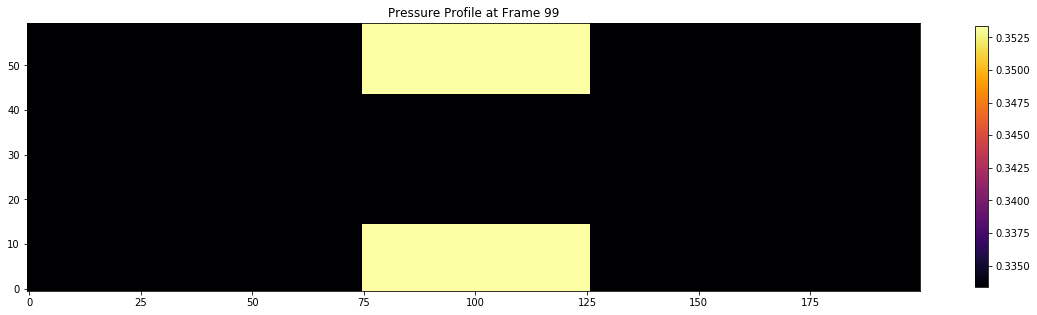
\includegraphics[width=0.85\textwidth]{pbc_pressure.png}
    \caption{Pressure field of the periodic channel.}
\end{figure}
The pressure field is everywhere around 0.333, which is consistent with the mass conservation in the periodic case. We then compare the average pressure with the average density. 
\begin{figure}[H]
    \centering
    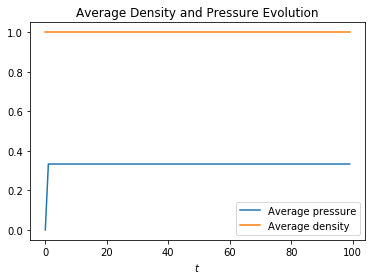
\includegraphics[width=0.5\textwidth]{HW2_solution/figs/pbc_prho.png}
    \caption{Time evolution of average density and average pressure.}
\end{figure}
Both density ($\rho=1$) and pressure ($p=\frac{1}{3}$) are conserved in this simulation, where the pressure value is approximately one-third of the density value. This coincides with the pressure-density relation in the setup:
$$p = c_s^2\rho=\frac{\rho}{3}$$

% ux
\begin{figure}[H]
    \centering
    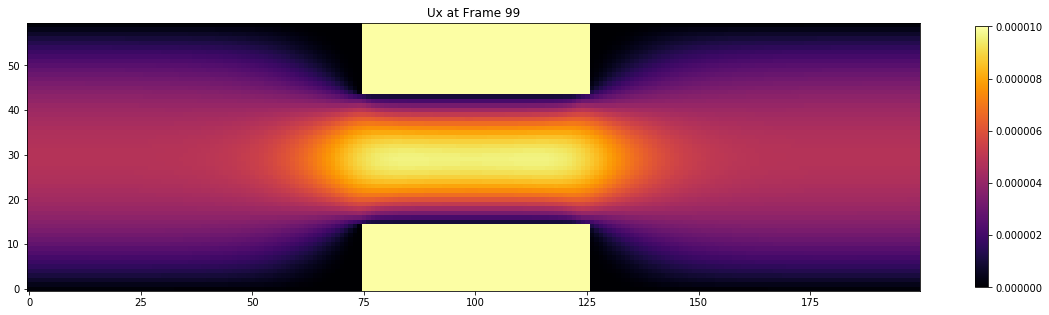
\includegraphics[width=0.85\textwidth]{pbc_ux.png}
    \caption{Velocity field in the x direction of the periodic channel.}
\end{figure}

% uy
\begin{figure}[H]
    \centering
    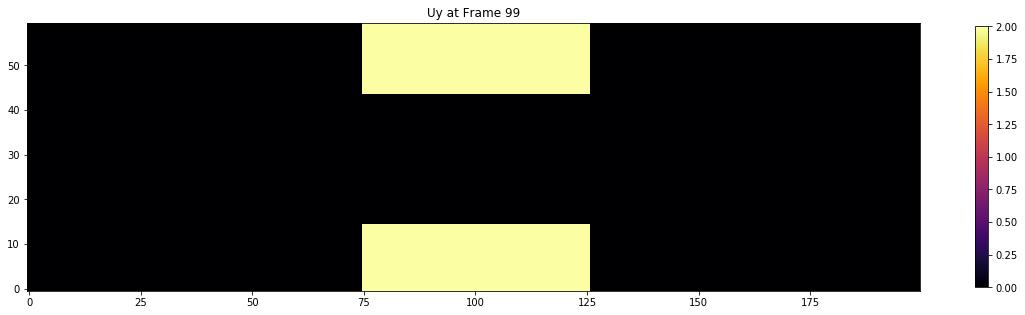
\includegraphics[width=0.85\textwidth]{pbc_uy.png}
    \caption{Velocity field in the y direction of the periodic channel.}
\end{figure}

We plot the velocity profile in both x and y direction along the y axis at $x=\frac{L}{2}$. Though encountering the narrowing, $u_x$ starts from transient and still develops into a parabolic shape, whereas $u_y$ is close to zero. This is consistent with the expected results of a periodic Poiseuille flow.
\begin{figure}[H]
    \centering
    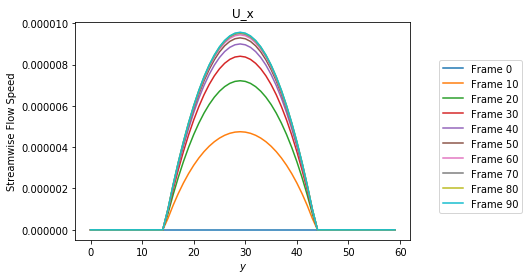
\includegraphics[width=0.49\textwidth]{HW2_solution/figs/pbc_ux_frame.png}
    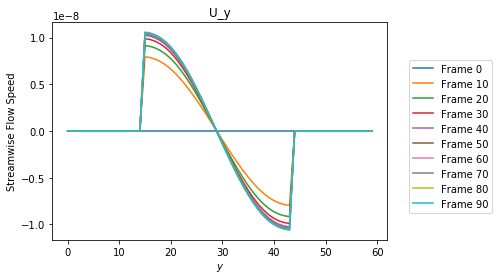
\includegraphics[width=0.46\textwidth]{HW2_solution/figs/pbc_uy_frame.png}
    \caption{Time evolution of average density and average pressure.}
\end{figure}

% speed
\begin{figure}[H]
    \centering
    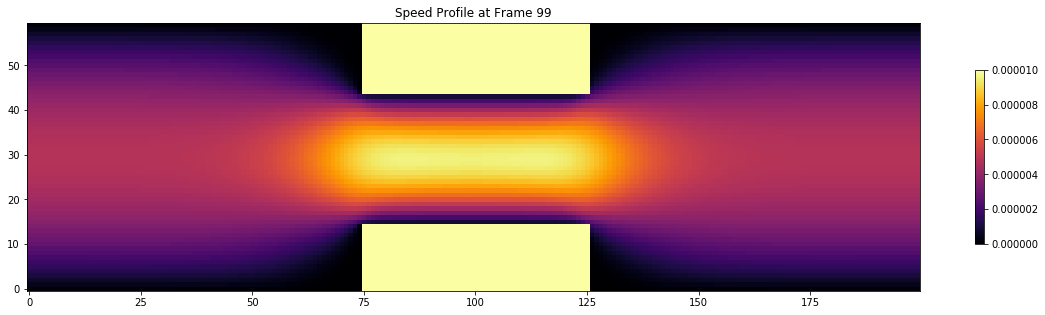
\includegraphics[width=0.85\textwidth]{pbc_speed.png}
    \caption{Velocity field of the periodic channel.}
\end{figure}
We can only compare the simulation results with the analytical solution of no narrowing. We use the last frame $u_x$ at $x=\frac{L}{2}$ since the Poiseuille flow is steady. Though the narrowing restricts the parabolic shape to develop, near the centerline the $u_x$ shows the parabolic shape that matches the analytical solution.
\begin{figure}[H]
    \centering
    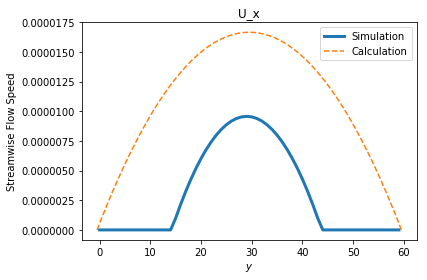
\includegraphics[width=0.5\textwidth]{HW2_solution/figs/pbc_ux_com.png}
    \caption{Simulation result vs. analytical solution of $u_x$.}
\end{figure}


We computed the speed $v$ in the channel and the volume flow rate $Q = \int_0^H v \: dy$ as a post-processing step in \tty{viz.ipynb}. At the last iteration, we have
\begin{align*}
    \overline{v} &= 0.000003 \\
    \max(v) &= 0.000010 \\
    Q &\approx 0.0001928
\end{align*}
The volume flow rate for steady state Poiseuille flow without the narrowing nor obstacle has the analytical form
$$Q = \frac{force D^3}{12\mu} \approx 0.00066$$
which is roughly three times the simulated volume flow rate. This is consistent with the one-third relation in the average velocity and maximum velocity. We plot the average and maximum velocity, along with the volume flow rate with respect to time, and the three quantities develop into steady state as the simulation goes in.
\begin{figure}[H]
    \centering
    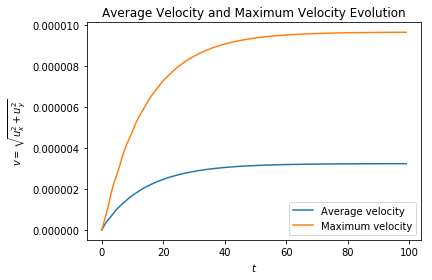
\includegraphics[width=0.5\textwidth]{HW2_solution/figs/pbc_speedavgmax.png}
    \caption{Time evolution of average velocity and maximum velocity.}
    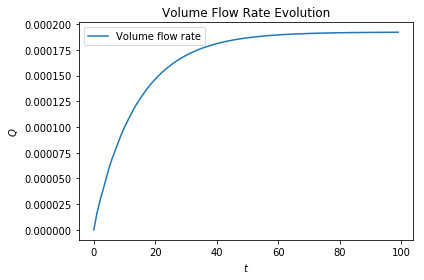
\includegraphics[width=0.5\textwidth]{HW2_solution/figs/pbc_vfrt.png}
    \caption{Time evolution of volume flow rate.}
\end{figure}





\textbf{II. Non-Periodic Channel} In the periodic case we fix the forcing term to introduce acceleration uniformly through the fluid. For the non-periodic case, we have an inlet and an outlet. By applying a uniform velocity at inlet and outlet with plug flow profiles, the flow will gradually become a steady Poiseuille flow because plug flow implies pressure gradient. For this particular visualization, we have
\begin{align}
    \textit{Re} &= 0.01 \\
    \nu &= \frac{2\tau - 1}{6} = 0.1 \Rightarrow \tau = 0.8 \\
    u_{max} &= \frac{\textit{Re}D}{\nu} = \frac{1}{60000} \\
    \mu &= \rho \nu = 0.1 \\
    \frac{dp}{dx} &= \frac{8\mu u_{max}}{D^2} = 3.7e-9 \\
    \Delta \rho = 3\Delta p &=3\frac{8\mu u_{max}}{D^2}L=2.22e-6 \\
    \rho_{inlet} &= \rho_0 + \frac{\Delta \rho}{2} \\
    \rho_{outlet} &= \rho_0 - \frac{\Delta \rho}{2}
\end{align}

% pressure
\begin{figure}[H]
    \centering
    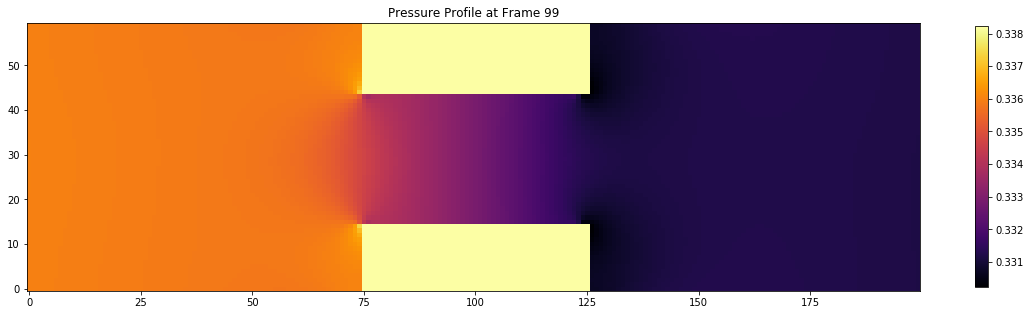
\includegraphics[width=0.85\textwidth]{lbm_mbc_pressure.png}
    \caption{Pressure field of the non-periodic channel.}
\end{figure}

% ux
\begin{figure}[H]
    \centering
    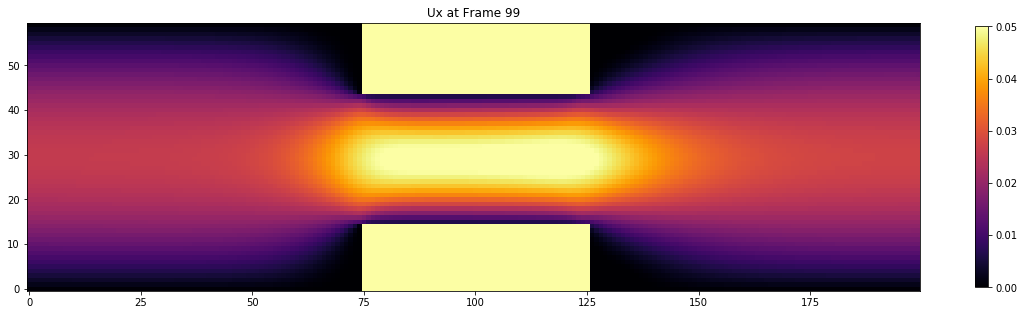
\includegraphics[width=0.85\textwidth]{lbm_mbc_ux.png}
    \caption{Velocity field in the x direction of the non-periodic channel.}
\end{figure}

% uy
\begin{figure}[H]
    \centering
    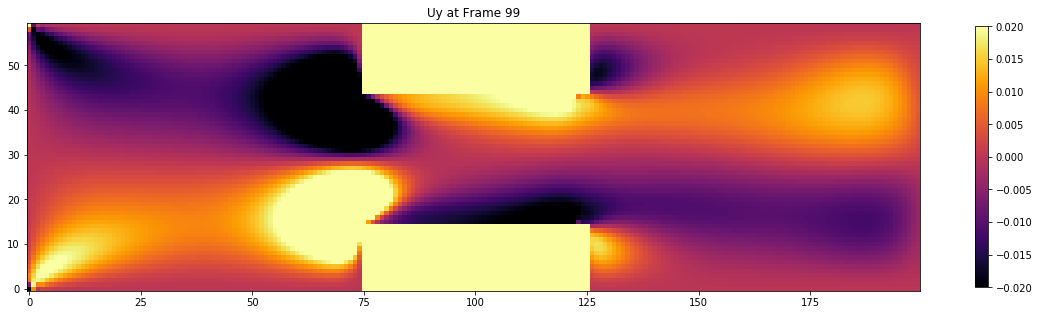
\includegraphics[width=0.85\textwidth]{lbm_mbc_uy.png}
    \caption{Velocity field in the y direction of the non-periodic channel.}
\end{figure}

% speed
\begin{figure}[H]
    \centering
    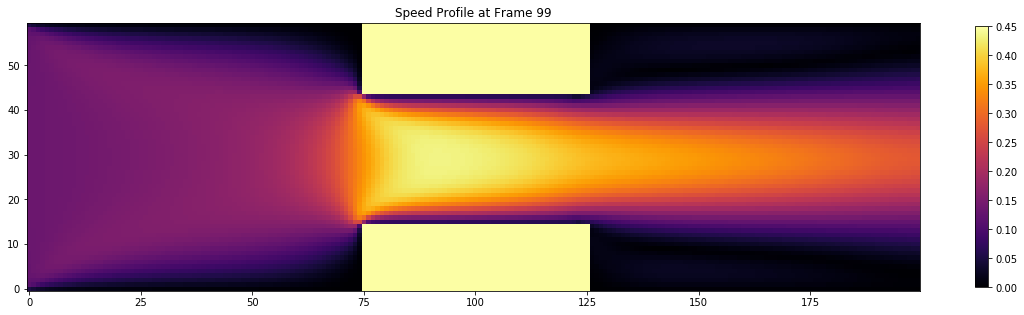
\includegraphics[width=0.85\textwidth]{lbm_mbc_speed.png}
    \caption{Velocity field of the non-periodic channel.}
\end{figure}

We also computed the speed $v$ in the channel and the volume flow rate $Q = \int_0^H v \: dy$ as a post-processing step in \tty{viz.ipynb}. At the last iteration, we have
\begin{align*}
    \overline{v} &= 0.017598 \\
    \max(v) &= 0.053161 \\
    Q &= 1.046670
\end{align*}

We computed the volume flow rate as the amount of fluid passing a vertical line
at a given value of $x$.  We would expect that this would be equal for any $x$ 
we chose at steady state by conservation of mass.  This is close to being true.
We therefore chose to take the mean of this quantity across all the $x$ values
in our grid to get the most accurate estimate of the volume flow.
As a sanity check, we printed out the volume flow every 20 steps from $x=0$ to 
$x=200$.  The results were all within 0.02 of the mean, except for the point
at x-100 in the middle of the inlet, where it was 0.08 below the mean. \\

Here are a few comments about these plots.
There is a significant difference in the scale of the speed and volume flow rate between
the periodic and non-periodic cases.
We have double checked our work and believe it to be correct.
The problem statement is in terms of a target Reynolds number, 
and the way we are calibrating the fluid speeds to achieve this is
quite different between the two cases.
We have confidence that each simulation is correct as presented. \\

The overall pressure profile is encouraging.  
The pressure varies only very slightly, as we expect for an incompressible fluid simulation.
The variations make sense too, as the modeled pressure is slightly higher on
the left and lower on the right.
The profile of the x-velocity $u_x$ is intuitive; the fluid needs to speed up
considerably in the narrowing for the flow to conserve mass.
We can also see it slowing down next to the boundary due to the 
no-slip boundary condition.
The y-velocity pattern shows very little flow in the y direction,
with four small pockets next to the four corners where the fluid
needs to narrow then widen out to pass through the narrow channel.
Overall these results make sense and look good to us.
Finally, we did a comparison of these results against the analytical
results for the PBC and found a good agreement.